\documentclass{article}\usepackage[]{graphicx}\usepackage[]{color}
%% maxwidth is the original width if it is less than linewidth
%% otherwise use linewidth (to make sure the graphics do not exceed the margin)
\makeatletter
\def\maxwidth{ %
  \ifdim\Gin@nat@width>\linewidth
    \linewidth
  \else
    \Gin@nat@width
  \fi
}
\makeatother

\definecolor{fgcolor}{rgb}{0.345, 0.345, 0.345}
\newcommand{\hlnum}[1]{\textcolor[rgb]{0.686,0.059,0.569}{#1}}%
\newcommand{\hlstr}[1]{\textcolor[rgb]{0.192,0.494,0.8}{#1}}%
\newcommand{\hlcom}[1]{\textcolor[rgb]{0.678,0.584,0.686}{\textit{#1}}}%
\newcommand{\hlopt}[1]{\textcolor[rgb]{0,0,0}{#1}}%
\newcommand{\hlstd}[1]{\textcolor[rgb]{0.345,0.345,0.345}{#1}}%
\newcommand{\hlkwa}[1]{\textcolor[rgb]{0.161,0.373,0.58}{\textbf{#1}}}%
\newcommand{\hlkwb}[1]{\textcolor[rgb]{0.69,0.353,0.396}{#1}}%
\newcommand{\hlkwc}[1]{\textcolor[rgb]{0.333,0.667,0.333}{#1}}%
\newcommand{\hlkwd}[1]{\textcolor[rgb]{0.737,0.353,0.396}{\textbf{#1}}}%
\let\hlipl\hlkwb

\usepackage{framed}
\makeatletter
\newenvironment{kframe}{%
 \def\at@end@of@kframe{}%
 \ifinner\ifhmode%
  \def\at@end@of@kframe{\end{minipage}}%
  \begin{minipage}{\columnwidth}%
 \fi\fi%
 \def\FrameCommand##1{\hskip\@totalleftmargin \hskip-\fboxsep
 \colorbox{shadecolor}{##1}\hskip-\fboxsep
     % There is no \\@totalrightmargin, so:
     \hskip-\linewidth \hskip-\@totalleftmargin \hskip\columnwidth}%
 \MakeFramed {\advance\hsize-\width
   \@totalleftmargin\z@ \linewidth\hsize
   \@setminipage}}%
 {\par\unskip\endMakeFramed%
 \at@end@of@kframe}
\makeatother

\definecolor{shadecolor}{rgb}{.97, .97, .97}
\definecolor{messagecolor}{rgb}{0, 0, 0}
\definecolor{warningcolor}{rgb}{1, 0, 1}
\definecolor{errorcolor}{rgb}{1, 0, 0}
\newenvironment{knitrout}{}{} % an empty environment to be redefined in TeX

\usepackage{alltt}
\usepackage[letterpaper, portrait, margin=1in]{geometry}
\IfFileExists{upquote.sty}{\usepackage{upquote}}{}
\begin{document}
\title{Problem Set 6}
\author{Jeffrey Kwarsick}
\maketitle
\section{Problem 1}
Below are the answers copied from the \emph{ps6\_question1.txt} in the \emph{ps6} folder on my github.
\begin{enumerate}
  \item The goals of the simulation study was to propose a test procedure of the work developed by Vuong.  Vuong derived a likelihood ratio test for model selection based on the information criterion by Kulback and Leibler.  This method was developed mainly for selecting models in multiple regression.  Therefore the goals of the simulation study were to test this procedure by lookingat a 1 component mixture vs. a 2 component normal mixture and a 2 component vs a 3 component normal mixture. Conclusions drawn from this test inform an empirical change to the statistic that appears to improve the rate of convergence of the limiting distribution.
  \item The authors decided to look at two of the most simple cases, a one and two component comparison and a two and three component comparison. They also decided on sample sizes that spanned from $10^1$ to $10^3$ with a 1000 simulations for each sample size.  Finally, they also chose different mixing proportions of the component distributions as well as the spacing between the components.  I think the size of the sample and the number of simulations run for each scenario would affect the statistical power of the method the most.  Small sample sizes and small number of replications (as referred in the paper) would reduce the statistical power, rather it would have a difficult time to detect a small effect if one existed.  The large sample size and number of replcations conducted would reduce the likelihood of missing even the smallest affect, and thereby increasing the statistical power.  I do not think there are data generating scenarios that the authors of this paper did not consider that would have been useful to consider.
  \item I do not think the tables presenting the results of the simulation results were not good at representing the results.  There are numerous amounts of the numbers reported, summarizing the simulation studies.  Given the number of results, I think that a more graphical representation would be better suited.  This would allow for easy comparison between results of different parameters and sample size.
  \item Based off of my assessment of the tables on power, Table 2 and Table 4, the results do make sense to me in terms of how the power varies as a function of the data generating mechanism.
  \item I think that the authors decided on 1000 simulations for their tests because 1000 simulations probably allowed the authors of the paper to be confident that the result of the simulations represent the true statistical properties of the theorem test.  I think that 10 simulations would not have been enough for this study.  We might decide that 1000 simulations is enough based off the what we consider to be an acceptable error required to accept or disprove a hypothesis question posed at the start of the simulation study.
\end{enumerate}
\section{Problem 2}
For this problem, I downloaded the stackoverflow database from the provided link to my local machine.  I first did some exploring around the database to identify the main tables within the database, as well as the fields within the tables.  I then used the \emph{RSQLite} package in order to create two lists and reduced them to only unqiue \emph{userids}.  One contained the \emph{userids} of the all the people that asked questions with the \emph{R} tag and the other contained the \emph{userids} of all the people that asked questions with the \emph{python} tag.  I then determined which \emph{userids} were unique to only both lists and and removed them from the list containing the userids of people only asking R-related questions. 
\par I completed this problem on my local desktop, a machine different than I am using to write up this homework.  I have uploaded a the script that I used to complete this problem to github.  It is called \emph{q2.R}.  The code is located below.
\begin{knitrout}
\definecolor{shadecolor}{rgb}{0.969, 0.969, 0.969}\color{fgcolor}\begin{kframe}
\begin{alltt}
\hlkwd{library}\hlstd{(RSQLite)}
\hlstd{drv} \hlkwb{<-} \hlkwd{dbDriver}\hlstd{(}\hlstr{"SQLite"}\hlstd{)}
\hlstd{dir} \hlkwb{<-} \hlstr{"C:/Users/Jeff/Documents/stat243/ps6"}
\hlstd{databFilename} \hlkwb{<-} \hlstr{'stackoverflow-2016.db'}
\hlstd{datab} \hlkwb{<-} \hlkwd{dbConnect}\hlstd{(drv,} \hlkwc{dbname} \hlstd{=} \hlkwd{file.path}\hlstd{(dir, databFilename))}

\hlcom{# test query}
\hlkwd{dbGetQuery}\hlstd{(datab,} \hlstr{"SELECT * FROM questions limit 5"}\hlstd{)}

\hlcom{# list tables}
\hlkwd{dbListTables}\hlstd{(datab)}

\hlcom{# List the fields within each table}
\hlkwd{dbListFields}\hlstd{(datab,} \hlstr{"questions_tags"}\hlstd{)}
\hlkwd{dbListFields}\hlstd{(datab,} \hlstr{"questions"}\hlstd{)}
\hlkwd{dbListFields}\hlstd{(datab,} \hlstr{"answers"}\hlstd{)}
\hlkwd{dbListFields}\hlstd{(datab,} \hlstr{"questionsAugment"}\hlstd{)}
\hlkwd{dbListFields}\hlstd{(datab,} \hlstr{"maxRepByQuestion"}\hlstd{)}
\hlkwd{dbListFields}\hlstd{(datab,} \hlstr{"users"}\hlstd{)}

\hlcom{# select all of the columns from the questions and questions id tables}
\hlcom{# where questionids are the same in both tables}
\hlcom{# where the tag = 'r'}
\hlstd{result1} \hlkwb{<-} \hlkwd{dbGetQuery}\hlstd{(datab,} \hlstr{"SELECT * from questions, questions_tags WHERE
                      questions.questionid = questions_tags.questionid AND 
                      tag = 'r'"}\hlstd{)}

\hlcom{# Look at the results of the test query}
\hlkwd{head}\hlstd{(result1)}

\hlcom{# query to pull the user ids from the users table}

\hlstd{result_r_questions} \hlkwb{<-} \hlkwd{dbGetQuery}\hlstd{(datab,} \hlstr{"SELECT distinct userid from 
                      questions Q, questions_tags T, users U
                      WHERE Q.questionid = T.questionid and Q.ownerid = U.userid
                      and tag = 'r'"}\hlstd{)}
\hlstd{result_py_questions} \hlkwb{<-} \hlkwd{dbGetQuery}\hlstd{(datab,} \hlstr{"SELECT distinct userid from 
                      questions Q, questions_tags T, users U
                      WHERE Q.questionid = T.questionid and Q.ownerid = U.userid
                      and tag = 'python'"}\hlstd{)}

\hlkwd{head}\hlstd{(result_r_questions)}
\hlkwd{head}\hlstd{(result_py_questions)}
\hlcom{# Convert data frames to vectors}
\hlstd{result_r} \hlkwb{<-} \hlkwd{unlist}\hlstd{(result_r_questions)}
\hlstd{result_py} \hlkwb{<-} \hlkwd{unlist}\hlstd{(result_py_questions)}
\hlcom{# Gives the unique list of userids}
\hlcom{# of people that have asked R questions}
\hlcom{# and no Python questions }
\hlstd{tmp} \hlkwb{<-} \hlkwd{setdiff}\hlstd{(result_r, result_py)}
\hlstd{num_only_r_users} \hlkwb{<-} \hlkwd{length}\hlstd{(tmp)}
\end{alltt}
\end{kframe}
\end{knitrout}
\section{Problem 3}
From problem three, I wanted to investigate the the following question -- 
\newline
\newline
\textbf{In the wake of the growing financial crisis that became a key focus of the 2008 U.S. Presidential Election, destabilized the global economy, and sunk the US economy into a substantial recession, how many people were looking up the cause of crisis, \emph{subprime lending}?}
\newline
\newline
I used an active session on \emph{savio2} in order to complete the initial processing using \emph{pySpark}. The code follows the demo session run during class.
\begin{knitrout}
\definecolor{shadecolor}{rgb}{0.969, 0.969, 0.969}\color{fgcolor}\begin{kframe}
\begin{alltt}
\hlcom{#Question 3 Problem Set 6}

dir      = \hlstr{'/global/scratch/paciorek/wikistats_full/dated/'}
home_dir = \hlstr{'/global/home/users/kwarsick/'}
\hlcom{#Import necessary packages/libraries}
from pyspark import SparkContext
sc = \hlkwd{SparkContext}()
import re
from operator import add

\hlcom{##Function to find search item of interest}
def \hlkwd{find}(line, regex = \hlstr{"Subprime_lending"}, language = None):
    vals = \hlkwd{line.split}(\hlstr{' '})
    if \hlkwd{len}(vals) < 6:
        \hlkwd{return}(False)
    tmp = \hlkwd{re.search}(regex, vals[3])
    if tmp is None \hlkwd{or} (language != None and vals[2] != language):
        \hlkwd{return}(False)
    else:
        \hlkwd{return}(True)

\hlcom{# find the file names}
lines = \hlkwd{sc.textFile}(dir) 		


\hlcom{#Collect search results in an object}
subprime_lending = \hlkwd{lines.filter}(find)\hlkwd{.repartition}(480)

\hlcom{# map-reduce step to sum hits across date-time-language triplets #}
    
def \hlkwd{stratify}(line):
\hlcom{    # create key-value pairs where:}
\hlcom{    #   key = date-time-language}
\hlcom{    #   value = number of website hits}
    vals = \hlkwd{line.split}(\hlstr{' '})
    \hlkwd{return}(vals[0] + \hlstr{'-'} + vals[1] + \hlstr{'-'} + vals[2], \hlkwd{int}(vals[4]))
	
	
spl_counts = \hlkwd{subprime_lending.map}(stratify)\hlkwd{.reduceByKey}(add)  \hlcom{# 5 minutes}
\hlcom{# 128889 for full dataset}

\hlcom{# map step to prepare output #}

def \hlkwd{transform}(vals):
\hlcom{    # split key info back into separate fields}
    key = vals[0]\hlkwd{.split}(\hlstr{'-'})
    \hlkwd{return}(\hlstr{","}\hlkwd{.join}((key[0], key[1], key[2], \hlkwd{str}(vals[1]))))

\hlcom{# output to file #}

\hlcom{# have one partition because one file per partition is written out}
outputDir = home_dir + \hlstr{'/'} + \hlstr{'spark-output'}
\hlkwd{spl_counts.map}(transform)\hlkwd{.repartition}(1)\hlkwd{.saveAsTextFile}(outputDir) \hlcom{# 5 sec.}
\end{alltt}
\end{kframe}
\end{knitrout}
This reduced the large dataset from 500GB to 53kB.  Below is the code used to plot the data collected on the Subprime Lending Wikipedia page.  The code is based off the Barack Obama search demo done in class.
\begin{knitrout}
\definecolor{shadecolor}{rgb}{0.969, 0.969, 0.969}\color{fgcolor}\begin{kframe}
\begin{alltt}
\hlkwd{library}\hlstd{(dplyr)}
\end{alltt}


{\ttfamily\noindent\itshape\color{messagecolor}{\#\# \\\#\# Attaching package: 'dplyr'}}

{\ttfamily\noindent\itshape\color{messagecolor}{\#\# The following objects are masked from 'package:stats':\\\#\# \\\#\#\ \ \ \  filter, lag}}

{\ttfamily\noindent\itshape\color{messagecolor}{\#\# The following objects are masked from 'package:base':\\\#\# \\\#\#\ \ \ \  intersect, setdiff, setequal, union}}\begin{alltt}
\hlkwd{library}\hlstd{(chron)}

\hlkwd{setwd}\hlstd{(}\hlstr{'/home/jkwarsick/Documents/STAT243_Fall2017/ps6-2017/'}\hlstd{)}

\hlstd{spl} \hlkwb{<-} \hlkwd{read.csv}\hlstd{(}\hlstr{'part-00000'}\hlstd{)}

\hlcom{#name four columns of list of lists}
\hlkwd{names}\hlstd{(spl)} \hlkwb{<-} \hlkwd{c}\hlstd{(}\hlstr{'date'}\hlstd{,}\hlstr{'time'}\hlstd{,}\hlstr{'lang'}\hlstd{,}\hlstr{'pagehits'}\hlstd{)}
\hlcom{#transform to characters for processing}
\hlstd{spl}\hlopt{$}\hlstd{date} \hlkwb{<-} \hlkwd{as.character}\hlstd{(spl}\hlopt{$}\hlstd{date)}
\hlstd{spl}\hlopt{$}\hlstd{time} \hlkwb{<-} \hlkwd{as.character}\hlstd{(spl}\hlopt{$}\hlstd{time)}
\hlcom{#corrects midnight times}
\hlstd{spl}\hlopt{$}\hlstd{time[spl}\hlopt{$}\hlstd{time} \hlopt  \hlkwd{c}\hlstd{(}\hlstr{"0"}\hlstd{,} \hlstr{"1"}\hlstd{)]} \hlkwb{<-} \hlstr{"000000"}
\hlstd{wh} \hlkwb{<-} \hlkwd{which}\hlstd{(}\hlkwd{nchar}\hlstd{(spl}\hlopt{$}\hlstd{time)} \hlopt{==} \hlnum{5}\hlstd{)}
\hlstd{spl}\hlopt{$}\hlstd{time[wh]} \hlkwb{<-} \hlkwd{paste0}\hlstd{(}\hlstr{"0"}\hlstd{, spl}\hlopt{$}\hlstd{time[wh])}
\hlcom{#creates combined list of date-time}
\hlstd{spl}\hlopt{$}\hlstd{chron} \hlkwb{<-} \hlkwd{chron}\hlstd{(spl}\hlopt{$}\hlstd{date, spl}\hlopt{$}\hlstd{time,}
                  \hlkwc{format} \hlstd{=} \hlkwd{c}\hlstd{(}\hlkwc{dates} \hlstd{=} \hlstr{'ymd'}\hlstd{,} \hlkwc{times} \hlstd{=} \hlstr{"hms"}\hlstd{))}
\hlcom{#switch to EST time}
\hlstd{spl}\hlopt{$}\hlstd{chron} \hlkwb{<-} \hlstd{spl}\hlopt{$}\hlstd{chron} \hlopt{-} \hlnum{5}\hlopt{/}\hlnum{24} \hlcom{# GMT -> EST}

\hlcom{#look only at the english data}
\hlstd{spl} \hlkwb{<-} \hlstd{spl} \hlopt \hlkwd{filter}\hlstd{(spl}\hlopt{$}\hlstd{lang} \hlopt{==} \hlstr{'en'}\hlstd{)}
\hlcom{#look at the peak of page hits}
\hlstd{sub} \hlkwb{<-} \hlstd{spl} \hlopt \hlkwd{filter}\hlstd{(spl}\hlopt{$}\hlstd{date} \hlopt{>} \hlnum{20081006} \hlopt{&} \hlstd{spl}\hlopt{$}\hlstd{date} \hlopt{<} \hlnum{20081010}\hlstd{)}

\hlcom{#pdf('subprime_lending_traffic.pdf', width = 5, height = 5)}
\hlkwd{par}\hlstd{(}\hlkwc{mfrow} \hlstd{=} \hlkwd{c}\hlstd{(}\hlnum{2}\hlstd{,} \hlnum{1}\hlstd{),} \hlkwc{mgp} \hlstd{=} \hlkwd{c}\hlstd{(}\hlnum{1.8}\hlstd{,} \hlnum{0.7}\hlstd{,} \hlnum{0}\hlstd{),} \hlkwc{mai} \hlstd{=} \hlkwd{c}\hlstd{(}\hlnum{0.6}\hlstd{,} \hlnum{0.6}\hlstd{,} \hlnum{0.1}\hlstd{,} \hlnum{0.1}\hlstd{))}
\hlkwd{plot}\hlstd{(spl}\hlopt{$}\hlstd{chron, spl}\hlopt{$}\hlstd{pagehits,} \hlkwc{type} \hlstd{=} \hlstr{'l'}\hlstd{,} \hlkwc{xlab} \hlstd{=} \hlstr{'Time'}\hlstd{,} \hlkwc{ylab} \hlstd{=} \hlstr{'Page Hits'}\hlstd{)}
\hlkwd{plot}\hlstd{(sub}\hlopt{$}\hlstd{chron, sub}\hlopt{$}\hlstd{pagehits,} \hlkwc{type} \hlstd{=} \hlstr{'l'}\hlstd{,} \hlkwc{xlab} \hlstd{=} \hlstr{'Time'}\hlstd{,} \hlkwc{ylab} \hlstd{=} \hlstr{'Page Hits'}\hlstd{)}
\hlkwd{points}\hlstd{(spl}\hlopt{$}\hlstd{chron, spl}\hlopt{$}\hlstd{pagehits)}
\end{alltt}
\end{kframe}
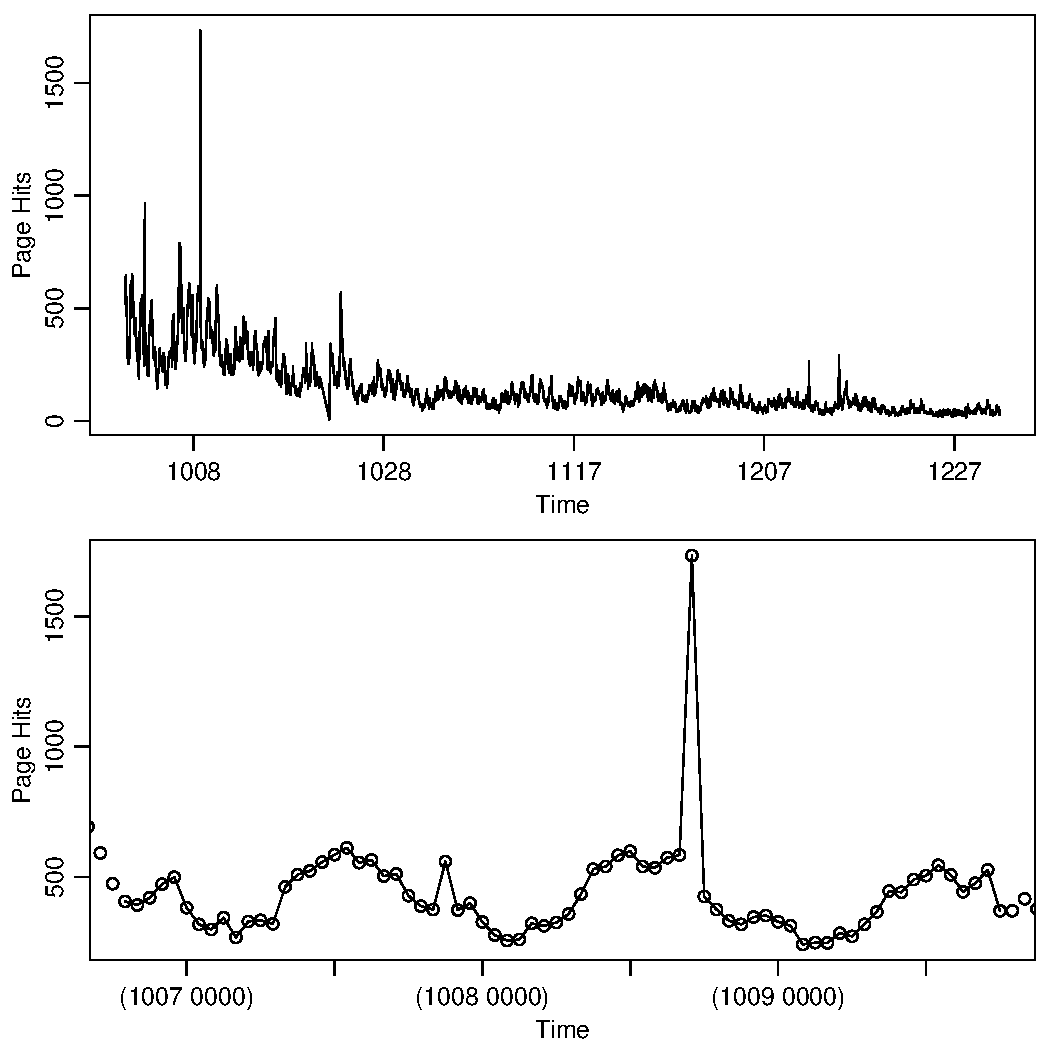
\includegraphics[width=\maxwidth]{figure/unnamed-chunk-3-1} 
\begin{kframe}\begin{alltt}
\hlcom{#dev.off()}
\end{alltt}
\end{kframe}
\end{knitrout}
The first plot shows the overall data of page hits on the 'Subprime Lending' Wikipedia page.  Compared to the demo in class on page hits for the Barack Obama, there are considerably fewer overall searches.  Most of the interesting observations for page hits on Subprime Lending came in early October.  This is shown to a greater detail in the second plot.  The traffic is considerably higher in page hits versus the rest of the two month time period.  
\par I conducted an online search to look into why the number of page hits reaches a maximum around October 8, 2008.  I found numerous articles that shed light on the likely reason for the spike.  In the days leading up the global maximum within the data, was frought with economic turmoil.  On October 6 - 7, 2008 the US Federal Government made over a trillion dollars available to inject into non-financial companies, nearly a trillion dollars into the banks, and the IRS ordered US corporations to liquidate capital overseas to inject in the American economy.  On the spike, on October 8, 2008, the US Federal Reserve along with other major world banks announced they would be reducing the lending rate by over 20\%, and the White House considered taking stakes in private banks.  This was all occuring during the worst week on Wallstreet since the Great Depression.  Since the spike in web traffic came around 5PM on October 8, 2008, it is reasonable to conclude that the move by the Federal Reserves and the other central banks to reduce the lending rate percentage was a clearly more significant sign of how dire the situation was becoming.  The roughly 1700 count maximum on this day also possibly denotes how only a small percentage of people were interested in the core issue of the crisis in the middle of it, and could possibly also mean that a majority of people did not understand the core of the problem and were far more concerned about the huge losses being taken on Wallstreet.  It is likely that the general public was entranced at the sheer amount of wealth, estimated in the trillions of US dollars, that was lost during this week and therefore were not concerned about the core issue.  It is also likely that the only a small number of people contributed the global maximum in the data because they were educated enough to investigate and understand the details of Subprime Lending.
\par All the information found was from a Wikipedia article, located below.
\newline
\newline
“Subprime crisis impact timeline.” \emph{Wikipedia}, Wikimedia Foundation, 15 Sept. 2017, 
\newline
en.wikipedia.org/wiki/Subprime\_crisis\_impact\_timeline\#2008.
\section{Problem 4}
\subsection{Part (a)}
I ran this problem as a batch submission.  The batch file is shown below.
\begin{knitrout}
\definecolor{shadecolor}{rgb}{0.969, 0.969, 0.969}\color{fgcolor}\begin{kframe}
\begin{alltt}
\hlcom{#!/bin/bash}
\hlcom{# Job name:}
\hlcom{#SBATCH --job-name=Q4Obama}
\hlcom{#}
\hlcom{# Account:}
\hlcom{#SBATCH --account=ic_stat243}
\hlcom{#}
\hlcom{# Partition:}
\hlcom{#SBATCH --partition=savio2}
\hlcom{# Request one node:}
\hlcom{#SBATCH--nodes=1}
\hlcom{#}
\hlcom{# Wall clock limit (1 hour 30 minutes here):}
\hlcom{#SBATCH --time=01:30:00}
\hlcom{#}
\hlcom{## Command(s) to run:}
module load r/3.2.5
R CMD BATCH --no-save obamaR.R obama.out
\end{alltt}
\end{kframe}
\end{knitrout}
The R-code that I used to run the same analysis as in the Spark class demo is shown below.
\begin{knitrout}
\definecolor{shadecolor}{rgb}{0.969, 0.969, 0.969}\color{fgcolor}\begin{kframe}
\begin{alltt}
\hlkwd{library}\hlstd{(}\hlstr{"readr"}\hlstd{)}
\hlkwd{library}\hlstd{(foreach)}
\hlkwd{library}\hlstd{(doParallel)}

\hlstd{concat_obama_results} \hlkwb{<-} \hlkwa{function}\hlstd{() \{}
  \hlcom{# path to Wikipedia web traffic}
  \hlstd{MY_PATH} \hlkwb{<-} \hlstr{"/global/scratch/paciorek/wikistats_full/dated_for_R/"}
  \hlcom{# find all the files in the directory}
  \hlstd{my_files} \hlkwb{<-} \hlkwd{list.files}\hlstd{(}\hlkwc{path}\hlstd{=MY_PATH,} \hlkwc{pattern}\hlstd{=}\hlstr{"part*"}\hlstd{)}
  \hlcom{# initiate multi-core processing}
  \hlstd{NCORES} \hlkwb{<-} \hlkwd{detectCores}\hlstd{(}\hlkwc{all.tests} \hlstd{=} \hlnum{FALSE}\hlstd{,} \hlkwc{logical} \hlstd{=} \hlnum{TRUE}\hlstd{)}
  \hlstd{cores} \hlkwb{<-} \hlkwd{makeCluster}\hlstd{(NCORES)}
  \hlkwd{registerDoParallel}\hlstd{(cores)}
  \hlcom{#output table}
  \hlstd{result_table} \hlkwb{=}
    \hlkwd{foreach} \hlstd{(}\hlkwc{i}\hlstd{=}\hlnum{1}\hlopt{:}\hlnum{96}\hlstd{,} \hlcom{# only did a small subset of the data}
             \hlkwc{.combine}\hlstd{=rbind,}
             \hlkwc{.packages}\hlstd{=}\hlkwd{c}\hlstd{(}\hlstr{'readr'}\hlstd{))} \hlopt \hlstd{\{}
               \hlkwd{library}\hlstd{(}\hlstr{"readr"}\hlstd{)}
               \hlcom{#reads in files, labels the lists within}
               \hlstd{to_add} \hlkwb{<-} \hlstd{readr}\hlopt{::}\hlkwd{read_delim}\hlstd{(}\hlkwd{paste}\hlstd{(MY_PATH, my_files[i],} \hlkwc{sep} \hlstd{=} \hlstr{""}\hlstd{),}
                                           \hlkwc{delim} \hlstd{=} \hlstr{" "}\hlstd{,}
                                           \hlkwc{col_names} \hlstd{=} \hlkwd{c}\hlstd{(}\hlstr{"date"}\hlstd{,} \hlstr{"time"}\hlstd{,} \hlstr{"language"}\hlstd{,}
                                                         \hlstr{"filename"}\hlstd{,} \hlstr{"site_hits"}\hlstd{,} \hlstr{"size"}\hlstd{)}
               \hlstd{)}
               \hlcom{# find and return lines related to Barack Obama}
               \hlkwd{return}\hlstd{(}\hlkwd{subset}\hlstd{(to_add,} \hlkwd{grepl}\hlstd{(}\hlstr{"Barack_Obama"}\hlstd{, filename)))}
               \hlkwd{gc}\hlstd{()}
             \hlstd{\}}
  \hlkwd{stopCluster}\hlstd{(c8)}
  \hlcom{#write out file to home directory}
  \hlkwd{write.table}\hlstd{(result_table,}
              \hlkwc{file} \hlstd{=} \hlstr{"~/Obama_Results.tsv"}\hlstd{,}
              \hlkwc{quote} \hlstd{=} \hlnum{FALSE}\hlstd{)}
\hlstd{\}}
\hlkwd{system.time}\hlstd{(}\hlkwd{concat_obama_results}\hlstd{())}
\end{alltt}
\end{kframe}
\end{knitrout}
This code was tested on a smaller subset of the data by downloading a single partition from the directory on savio and splitting it on my local machine.  After, it was ran as a batch run submission.  I ran into several issues regarding reaching the step memory limit of the node that I had access to.  I attempted to apply some of the changes based on posts from Piazza but still ran into the same problems.  In the end, I elected to run the code on a subset of the data files.  This subset is only one tenth of the 960 total files.  
\subsection{Part (b)}
Since the processing of 96 of the files, or 10\% of the total files, took roughly 9 (8.8) minutes, scaling to the total numbers of the files would take roughly 90 (88) minutes.  If I were to use 4 nodes to complete this task the total time would take 22 minutes.  Compared to the 15 minutes taken by Spark running on 4 cores, R is comparable to Spark in this case..
\subsection{Part (c)}
\begin{knitrout}
\definecolor{shadecolor}{rgb}{0.969, 0.969, 0.969}\color{fgcolor}\begin{kframe}
\begin{alltt}
\hlkwd{library}\hlstd{(readr)}
\hlkwd{library}\hlstd{(foreach)}
\hlkwd{library}\hlstd{(doParallel)}
\hlkwd{library}\hlstd{(doMC)}

\hlstd{concat_obama_results_preschedule} \hlkwb{<-} \hlkwa{function}\hlstd{() \{}
  \hlcom{# path to Wikipedia web traffic}
  \hlstd{MY_PATH} \hlkwb{<-} \hlstr{"/global/scratch/paciorek/wikistats_full/dated_for_R/"}
  \hlcom{# find all the files in the directory}
  \hlstd{my_files} \hlkwb{<-} \hlkwd{list.files}\hlstd{(}\hlkwc{path}\hlstd{=MY_PATH,} \hlkwc{pattern}\hlstd{=}\hlstr{"part*"}\hlstd{)}
  \hlcom{# initiate multi-core processing}
  \hlcom{# enable prescheduling}
  \hlstd{mcoptions} \hlkwb{<-} \hlkwd{list}\hlstd{(}\hlkwc{preschedule}\hlstd{=}\hlnum{TRUE}\hlstd{)}
  \hlstd{NCORES} \hlkwb{<-} \hlkwd{detectCores}\hlstd{(}\hlkwc{all.tests} \hlstd{=} \hlnum{FALSE}\hlstd{,} \hlkwc{logical} \hlstd{=} \hlnum{TRUE}\hlstd{)}
  \hlstd{cores} \hlkwb{<-} \hlkwd{makeCluster}\hlstd{(NCORES)}
  \hlkwd{registerDoParallel}\hlstd{(cores)}
  \hlcom{#output table}
  \hlstd{result_table} \hlkwb{=}
    \hlkwd{foreach} \hlstd{(}\hlkwc{i}\hlstd{=}\hlnum{1}\hlopt{:}\hlnum{96}\hlstd{,}
             \hlkwc{.combine}\hlstd{=rbind,}
             \hlkwc{.packages}\hlstd{=}\hlkwd{c}\hlstd{(}\hlstr{'readr'}\hlstd{),}
             \hlkwc{.options.multicore}\hlstd{=mcoptions)} \hlopt \hlstd{\{}
               \hlkwd{library}\hlstd{(}\hlstr{"readr"}\hlstd{)}
               \hlcom{#reads in files, labels the lists within}
               \hlstd{to_add} \hlkwb{<-} \hlstd{readr}\hlopt{::}\hlkwd{read_delim}\hlstd{(}\hlkwd{paste}\hlstd{(MY_PATH, my_files[i],} \hlkwc{sep} \hlstd{=} \hlstr{""}\hlstd{),}
                                           \hlkwc{delim} \hlstd{=} \hlstr{" "}\hlstd{,}
                                           \hlkwc{col_names} \hlstd{=} \hlkwd{c}\hlstd{(}\hlstr{"date"}\hlstd{,} \hlstr{"time"}\hlstd{,} \hlstr{"language"}\hlstd{,}
                                                         \hlstr{"filename"}\hlstd{,} \hlstr{"site_hits"}\hlstd{,} \hlstr{"size"}\hlstd{)}
               \hlstd{)}
               \hlcom{# find and return lines related to Barack Obama}
               \hlkwd{return}\hlstd{(}\hlkwd{subset}\hlstd{(to_add,} \hlkwd{grepl}\hlstd{(}\hlstr{"Barack_Obama"}\hlstd{, filename)))}
               \hlkwd{gc}\hlstd{()}
             \hlstd{\}}
  \hlkwd{stopCluster}\hlstd{(c8)}

  \hlkwd{write.table}\hlstd{(result_table,}
              \hlkwc{file} \hlstd{=} \hlstr{"~/Obama_Results.tsv"}\hlstd{,}
              \hlkwc{quote} \hlstd{=} \hlnum{FALSE}\hlstd{)}
\hlstd{\}}

\hlkwd{system.time}\hlstd{(}\hlkwd{concat_obama_results_preschedule}\hlstd{())}
\end{alltt}
\end{kframe}
\end{knitrout}
Due to time constraints, I did not have a chance to run the code above to see the affects of prescheduling.
\par In this case, I would expect it to not make a difference in this case.
\section{Problem 5}
\subsection{Part (a)}
This part is has been handwritten.  In order to understand and complete this part of the problem,  I found and referred to the paper cited below.  The result is consistent with the result from class.
\newline
\newline
Reference Citation: Floating Point Operations in Matrix-Vector Calculus (v. 1.3). Raphael Hunger. Technical Report. 2007.
\subsection{Part (b)}
Because the Cholesky Decomposition does not refer to preceding rows during computation, it is acceptable to overwrite as you conduct the decomposition.  It will not interfere with future computations in the decomposition, therefore it is fine to save the upper triangular matrix in the memory block of the original matrix, overwriting the original in the process.
\end{document}
